
\newcommand{\dgrs}{$^{\circ}$}

\section{Relative pose tracking}

We have seen that a gentle tap can be enough to reveal the outline of
an object in the image plane.  For very asymmetric objects, the
outline can be enough to greatly constrain their 3D pose.  For more
symmetric objects, the outline is not enough, and appearance or
tactile information needs to be considered.  Such information is
likely to be available only sporadically, depending on whether particular
surface features or in view or whether the robot arm is in contact
with the object.  This section describes a pose representation
that is well suited to ``piece-meal'' approaches.

We can decompose the three-dimensional processes involved in
determining the appearance of an object into an interaction between
two 2D objects: the image plane, and the surface of the object.  At
any moment, some set of surface patches on the object will be parallel
to the image plane.  As the object rotates in depth, different patches
become parallel.  When the object translates, or rotates in plane, the
parallel patches remain constant.  Figure~\ref{fig:tracking-dofs}
shows this decomposition.

\begin{figure}[tbp]
\centerline{\includegraphics[width=\columnwidth]{tracking-dofs.eps}}
\caption{ 
%
  Two-dimensional tracking; four degrees of freedom are straightforward,
  but the last two are a little trickier.
%
}
\label{fig:tracking-dofs}
\end{figure}


\subsection{Current results}

The system has so far been tested on a data-set made available by
Sclaroff et al~\cite{lacascia00fast}, consisting of video of head
movements with ground truth measured by a Flock of Birds sensor on the
subjects' heads.  These sequences are 200 frames in duration.  To test
the stability of the tracker over long intervals, the Sclaroff
sequences are here artificially extending by looped them forward and
back for twenty iterations.  Angular measurements are limited by the
accuracy with which they can be initialized, which turns out to be to
within about 5\dgrs\ for roll and yaw, and about 10\dgrs\ for pitch.

\begin{figure}[tbp]
\centerline{\includegraphics[width=\columnwidth]{yaw-roll-result.eps}}
\centerline{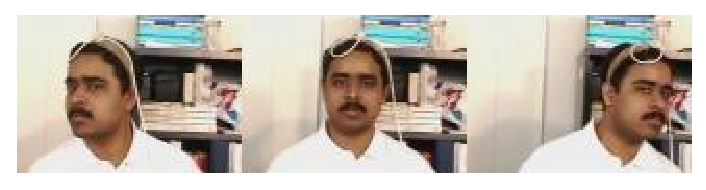
\includegraphics[width=\columnwidth]{yaw-extremes.eps}}
\caption{ 
%
  Results for a sequence containing a yaw movement and horizontal
  translation, with all other parameters remaining basically unchanged
  except for a slight roll.  The top row shows ground truth.  The
  second row shows the estimated pose parameters that change
  significantly during the sequence.  The estimated $x$ coordinate is
  left in terms of the image plane.  Values plotted are averaged for
  each occurrence of a particular frame over a {\em single tracking
    run} constructed from a 200-frame sequence being played, then
  played in reverse, then repeated again for twenty iterations.  Error
  bars show the standard deviation of estimates for each frame.
%
}
\label{fig:yaw-roll-result}
\end{figure}
